\section{Austenitic Steels and Radiation Damage in Generation III+ and IV Reactors}

\subsection{Atom Damage Cascades}

Fission fragments carry away the majority of the energy released during fission, with an approximate energy of 170MeV per 235U fission event.  The fragments are large and have a highly charged positive nucleus that stops rapidly due to the Coulomb interaction with the nuclei of surrounding atoms.  Electrons released by beta decay travel a greater distance; they lose energy by interacting with electrons, but may also knock atoms out of place.  Neutrons travel further still and lose energy by interacting directly with the nuclei of the surrounding material.

When an incoming projectile hits an atom, the primary knock-on atom (PKA), this is knocked out of its place and loses energy by colliding with other atoms and to the electrons in the metal.  Depending on the energy of the PKA, this causes a damage cascade.  Atoms knocked out of their regular position in the crystal lattice leave vacancies behind.  The displaced atoms either recombine with vacancies, become interstitial atoms or diffuse to defect sinks.

A number of complex problems arise as a result of this damage.


\subsection{Damage Rates}

The safety of a Nuclear reactor is the primary concern; it must generate power, but it must be safe.  It must also be cost efficient.  Generation II PWR fuel assembles were expected to withstand several DPA\cite{genIVstrucmat}.  In BWRs the materials are designed to be irradiated by $10^22 n/cm^2/s$, experiencing approximately 7 DPA over the lifetime of the components\cite{lightwaterallenbusby}.  Components in PWRs are irradiated by up to $10^22 n/cm^2/s$, and are expected to operate up to an irradiation dose of 70 dpa\cite{lightwaterallenbusby}.  To remain cost efficient, components in Gen IV reactors will be expected to operate safely up to even higher doses or irradiation damage.  Components in sodium-cooled fast reactors will be expected to withstand up to 200 DPA over their lifetime to meet the requirements of cost effectiveness and durability\cite{genIVstrucmat}.

Neutrons given out during 235U fission range from 0 to 14 MeV, and the energy transferred to a target atom depends on the scattering angle of the neutron and the mass of the target nucleus.  

\begin{equation}
\begin{split}
\alpha = (\frac{m_N-1}{m_N+1})^2 \\
E_N = E_n (1 - \frac{(1+\alpha) + (1 - \alpha) cos \theta_C}{2})
\end{split}
\label{eq:eqNeutronEnergyTransfer}
\end{equation}


The 

\begin{figure}
\centering
\begin{subfigure}{.5\textwidth}
  \centering
  \includegraphics[width=.4\linewidth]{chapters/background_austenitic_steels_in_nuclear/plots/scattering_angle.eps}
  \caption{A subfigure}
  \label{fig:sub1}
\end{subfigure}
\begin{subfigure}{.5\textwidth}
  \centering
  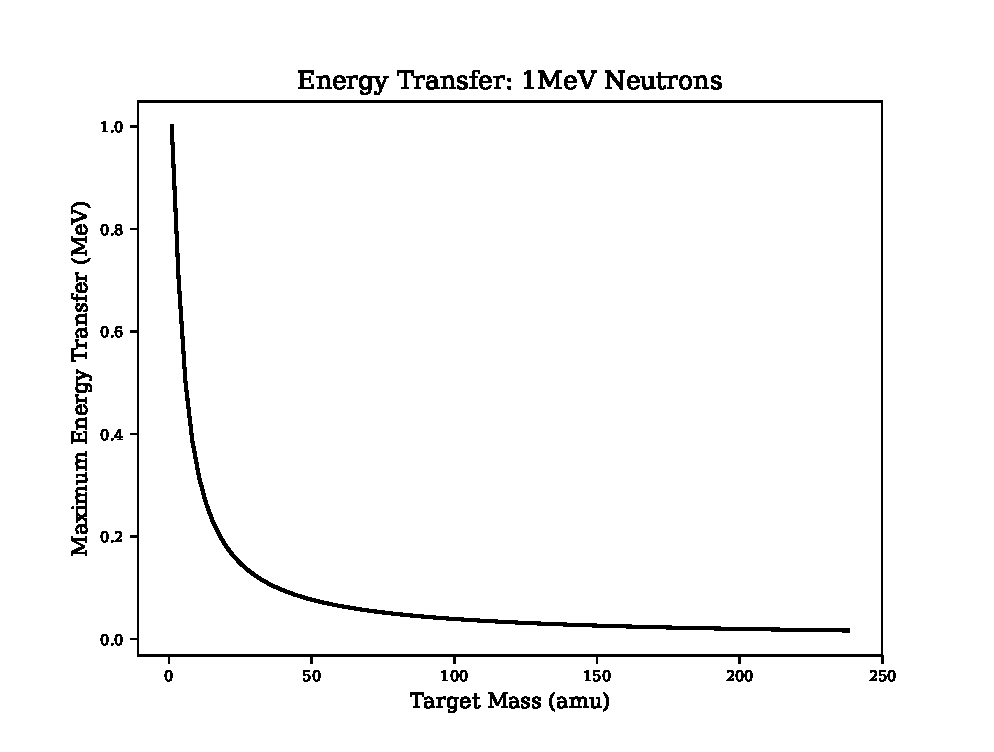
\includegraphics[width=.4\linewidth]{chapters/background_austenitic_steels_in_nuclear/plots/nuclei_mass.eps}
  \caption{A subfigure}
  \label{fig:sub2}
\end{subfigure}
\caption{A figure with two subfigures}
\label{fig:test}
\end{figure}









\subsection{Swelling}




\subsection{Radiation Induced Segregation}

The diffusion of atoms within an alloy has an impact on the characteristics of the metal \cite{nickeldiffusion}.  When radiation causes point defects, these interstitials also diffuse parallel to thermal solute diffusion.  At low temperatures, the atoms are unable to diffuse at an appreciable rate; the mobility of vacancies are low\cite{gswas} and there are an excess of vacancies due to radiation damage, and this leads to recombination of defects.  At high temperatures, there is a higher concentration of thermal defects\cite{lightwaterallenbusby}.  This increases the defect recombination rate and reduces migration of defects to sinks, such as grain boundaries.

The melting temperature range of 304 and 316 stainless steel are approximatelyh 1695-1722K and 1644-1672K respectively.  Generation II reactors, such as Sizewell B, have an operating temperature of several hundred degrees centigrade.  The inlet temperature for the Sizewell B PWR reactor is 566K\cite{sizewellbtemp} and the outlet temperature is 597K\cite{sizewellbtemp}.  Operating at approximately 35% the melting point of the steel, this is, unfortunately, a good temperature for radiation induced segregation to occur.

\begin{figure}[h]
  \begin{center}
    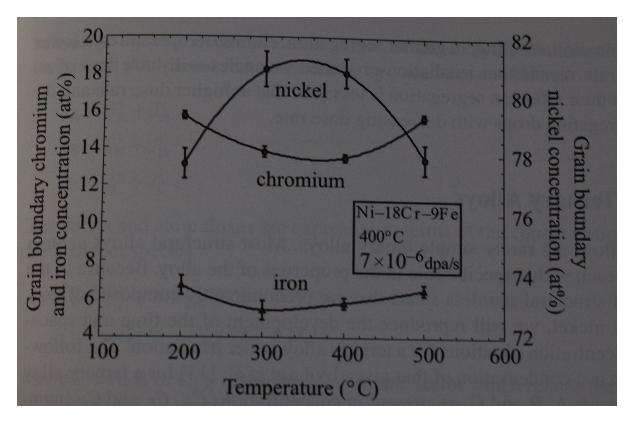
\includegraphics[scale=0.70]{chapters/background_austenitic_steels_in_nuclear/plots/nicrfeseg.eps}[scale=0.6]
    \caption{Graph caption}
    \label{graph:graph1}
  \end{center}
\end{figure}

The Kirkendall effect concerns the diffusion of one material into another and vice versa at an interface.  In the original experiment performed by Kirkendall and Smigelskas, brass (Cu and Zn) was sandwiched between copper and left at a temperature of over 1050K for almost two months.  Using Molybdenum as a marker, it was discovered that zinc diffused out of the brass faster than the copper diffused into the brass.  

The inverse Kirkendall effect is driven by an external force, such as irradiation.



\begin{figure}[h]
  \begin{center}
    \includegraphics[scale=0.70]{chapters/background_austenitic_steels_in_nuclear/images/crseg.png}[scale=0.6]
    \caption{Graph caption}
    \label{graph:graph1}
  \end{center}
\end{figure}



\subsection{Irradiation Hardening}



